\chapter{Geometrisk Optik} \label{cha:Optik}

\section{Introduktion}
I geometrisk optik bruger man en simpel model for lys, hvor lyset beskrives som stråler, der bevæger sig i lige linjer. Denne model siger ikke noget om den præcise natur af lyset, men sammen med nogle få love er den tilstrækkelig til at give en beskrivelse af både refleksion og refraktion (brydning) af lys. På figur \ref{ind_ud_og_obj_img_def} del A) er der vist et eksempel på en indgående lysstråle, der reflekteres og brydes ved en overflade mellem to materialer. Der er også tegnet en stiplet linje på figuren, som er vinkelret på overfladen. En sådan linje kaldes for overfladens normal, og den bruges som en reference til at måle indgangsvinklen $\theta_a$, refleksionsvinklen $\theta_r$ og brydningsvinklen $\theta_b$, der også er vist på figuren. Disse processer er beskrevet ved de følgende to love.\\

\noindent
\textbf{Refleksionsloven}: Denne lov siger, at når en lysstråle reflekteres ved en overflade, så vil indgangsvinklen være lig refleksionsvinklen:
\begin{equation}
\theta_a = \theta_r
\end{equation}
\textbf{Brydningsloven}: Denne lov siger, at når en lysstråle brydes ved overgangen mellem to forskellige materialer $a$ og $b$, så er forholdet mellem indgangsvinklen og brydningsvinklen beskrevet ved den følgende formel\footnote{Nogle gange kaldes denne lov også for Snells Lov.}:
\begin{equation}
n_a \sin(\theta_a) = n_b \sin(\theta_b) 
\label{bryd_lov}
\end{equation}
Her er $n_a$ og $n_b$ brydningsindekserne for de to materialer. Brydningsindekset for et materiale er defineret som
\begin{equation}
n = \frac{c}{v},
\end{equation}
hvor $c$ er lysets fart i vakuum, og $v$ er lysets fart i materialet. I en mere komplet model, hvor lyset beskrives som elektromagnetiske bølger, kan man udlede begge disse love, men her vil de blot blive betragtet som eksperimentelle resultater.\\

Udover disse to love og vores simple model for lyset, er der to andre koncepter, som er helt centrale for geometrisk optik. Det første er konceptet om et \textit{objekt}, hvilket her defineres som enhver form for genstand, der kan udsende eller reflektere lys. Det andet er konceptet om et \textit{billede}, der er den reflekterede eller brudte version af objektet, som en observatør rent faktisk ser. Der er vist et eksempel på figur \ref{ind_ud_og_obj_img_def} del B), som illustrerer de to koncepter.
\begin{figure}[h!]
	\centering
	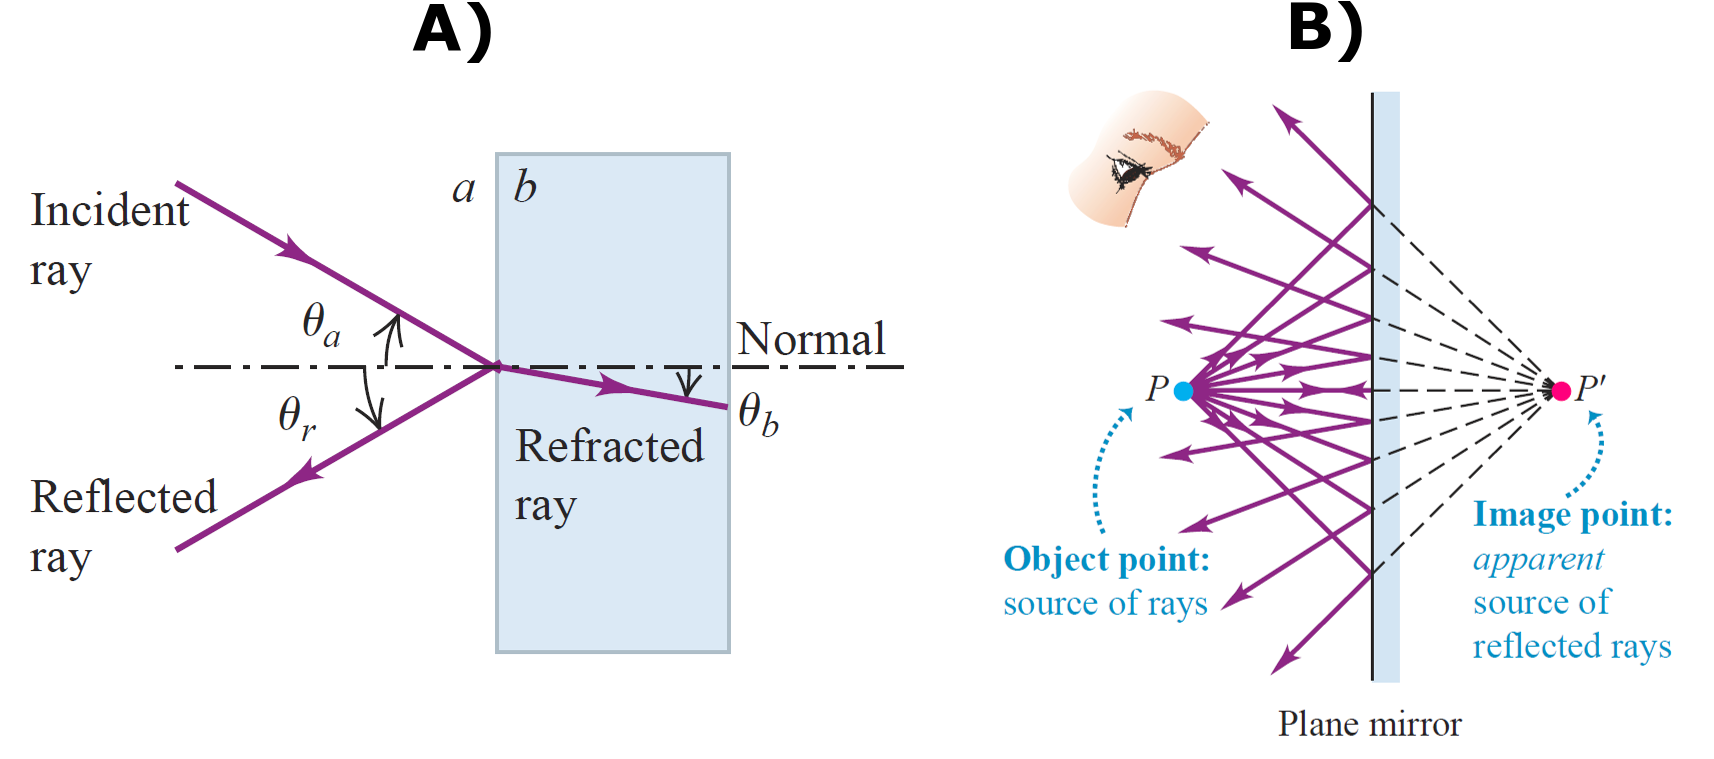
\includegraphics[scale=0.22]{Geometrisk-Optik/ind_ud_og_obj_img_def.PNG}
	\caption{På figurens del A) ses en indkommende lysstråle, der reflekteres og brydes ved overgangen mellem to materialer $a$ og $b$. På del B) ses et punktobjekt placeret i punktet $P$ og objektets billede i punktet $P'$, der er dannet af spejlet. Billedpunktet $P'$ er som illustreret det punkt, hvor observatøren ser objektet være.}
	\label{ind_ud_og_obj_img_def}
\end{figure}

\section{Billeddannelse}

\subsection*{Billeddannelse ved Fladt Spejl}

Som et første eksempel på billeddannelse betragtes et simpelt punktobjekt (et objekt uden en fysisk udstrækning), der placeres i nærheden af et fladt spejl, som det er vist på figur \ref{billeddannelse_flad_og_pil} del A). Her er $s$ afstanden mellem objektet og spejlet, der kaldes for objektafstanden, mens $s'$ er afstanden mellem billedet og spejlet, der kaldes billedafstanden. Derudover er der de to punkter, $P$ og $P'$, der angiver placeringen af objektet og billedet, og som derfor kaldes for henholdsvis objekt- og billedpunktet. På figuren er der også vist et eksempel på en lysstråle, der danner en vinkel $\theta$ i forhold til overfladens normal (stiplede linje). Det centrale at bemærke her er, at man lige så godt kunne have valgt en hvilken som helts anden vinkel $\theta'$, og man ville stadig have det samme billedpunkt.\\  

Når man skal arbejde med objekt- og billedafstandene, $s$ og $s'$, er der nogle fortegnskonventioner, som man skal huske at følge. Disse er givet ved de første 2 af de følgende regler. Den 3. regel er ikke relevant for eksemplet her med et fladt spejl, men den bliver vigtig, når man skal arbejde med refleksion og brydning ved krumme overflader. De 3 regler er som følger:\\

\noindent
1. \textbf{Regl for objektafstand:} Når et objekt er på samme side af den reflekterende eller brydende overflade som den indkommende lysstråle, er objektafstanden $s$ positiv. Ellers er den negativ.\\

\noindent
2. \textbf{Regl for billedafstand:} Når et billede er på samme side af den reflekterende eller brydende overflade som den udgåede lysstråle, er billedafstanden $s'$ positiv. Ellers er den negativ.\\

\noindent
3. \textbf{Regl for krumningsradius af en sfærisk overflade:} Når krumningscentrummet $C$ er på samme side som den udgående lysstråle, er krumningsradiusen $r$ positiv. Ellers er den negativ.\\

Kigger man igen på eksemplet med et fladt spejl, ser man hurtigt, at objektet altid vil være på samme side som den indgående lysstråle, og at billedet altid vil ligge på den anden side af den udgående lysstråle. Derfor kan man for et fladt spejl give følgende resultat:
\begin{equation}
s = -s' \quad \quad \quad \left( \text{for fladt spejl} \right)
\label{obj_img_fladt}
\end{equation}

\begin{figure}[h!]
	\centering
	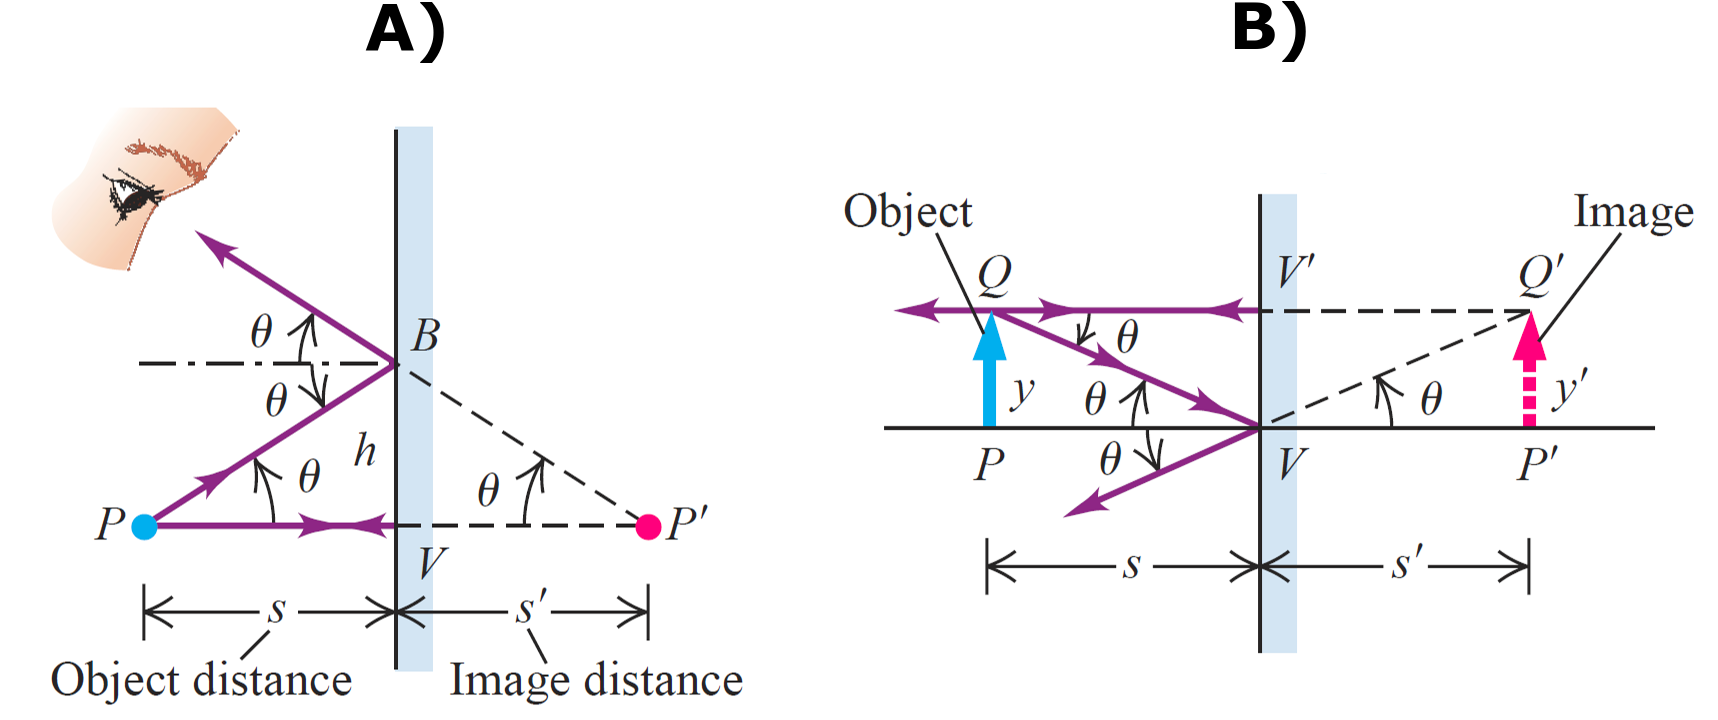
\includegraphics[scale=0.23]{Geometrisk-Optik/billeddannelse_flad_og_pil.PNG}
	\caption{På figurens del A) ses et punktobjekt og billedobjekt ved et fladt spejl samt objektafstanden $s$ og billedafstanden $s'$. På del B) ses en pil i blå der udgør objektet, som her har en udstrækning, mens billedet af objektet er angivet med den lyserøde pil, der også har en udstrækning. Også her er der angivet objekt- og billedafstand.}
	\label{billeddannelse_flad_og_pil}
\end{figure}
Selvom dette simple eksempel giver en god illustration af nogle af de grundlæggende begreber i geometrisk optik, er det ikke et særligt realistisk eller relevante eksempel, da punktobjekter ikke findes ude i naturen. Det er derfor oplagt at kigge på et lidt mere generelt tilfælde, hvor objektet har en fysisk udstrækning. Et eksempel på dette kan være en pil med en given længde $y$, som det er vist i figur \ref{billeddannelse_flad_og_pil} del B). Her ses det, at når man har et objekt med en udstrækning $y$, så får man også et billede med en udstrækning $y'$. I dette eksempel består objektet af alle punkter på linjen $PQ$, mens billedet består af alle punkter på linjen $P'Q'$. Kigger man på et enkelt punkt af objektet, f.eks $Q$, ser man også, at dette punkt svarer til et enkelt punkt af billedet, hvor det her er $Q'$. Altså vil en observatør, på samme side af spejlet som den indgående lysstråle, se pilespidsen ligge i punktet $Q'$ og ikke $Q$. En vigtig ting her er, at ligesom med $s$ og $s'$, så er der også en fortegnskonvention for størrelserne $y$ og $y'$. Denne konvention siger blot, at hvis objekt- og billedpilen peger i samme retning, så er $y$ og $y'$ positive, mens hvis objekt- og billedpilen peger i modsatte retninger, så er $y$ positiv og $y'$ er negativ.\\

Når man arbejder med objekter og billeder, der har en udstrækning, definerer man typisk en tværgående forstørrelse $m$ som forholdet mellem højden af billedet og objektet på følgende måde:
\begin{equation}
m = \frac{y'}{y}
\end{equation}
Benytter man fortegnskonventionen for $y$ og $y'$, ses det, at hvis objekt- og billedpilen peger i samme retning, så er $m$ positiv, og hvis de peger i modsatte retninger er $m$ negativ. Kigger man igen på figur \ref{billeddannelse_flad_og_pil} del B), kan man se, at objekt- og billedpilen altid vil pege i samme retning for et fladt spejl, og at $y$ og $y'$ vil være lige store. Dette giver altså følgende resultat
\begin{equation}
m = +1 \quad \quad \quad \left( \text{for fladt spejl} \right)
\end{equation}
Som det ses i de to gennemgåede eksempler ovenover, er det muligt at danne billeder af både punktobjekter og objekter med udstrækning ved et fladt spejl. Det er dog begrænset, hvor anvendeligt dette er, da man ikke kan variere den tværgående forstørrelse $m$, hvilket er essentielt, hvis man vil bruge geometrisk optik, til at lave forskellige teknologier som mikroskoper eller teleskoper. For at opnå denne frihed til at variere $m$, må man gå væk fra det simple tilfælde med et fladt spejl, og i stedet kigge på refleksion og brydning ved krumme overflader.  

\subsection*{Billeddannelse ved Krumme Overflader}

Det næste man kan kigge på indenfor geometrisk optik er, hvad der sker, hvis man skifter det flade spejl ud med et spejl med en krum overflade. Som et første eksempel er det oplagt at kigge på et hulspejl, hvor spejlet består af et udsnit af en cirkel, som det er vist på figur \ref{billeddannelse_krum}. Her er $R$ cirklens radius, $C$ kaldes for krumningscentrummet og ligger i cirklens centrum, $V$, der ligger i spejlets centrum, kaldes for spejlets vertex og den vandrette streg langs $CV$ kaldes for den optiske akse. 
%
\begin{figure}[h!]
	\centering
	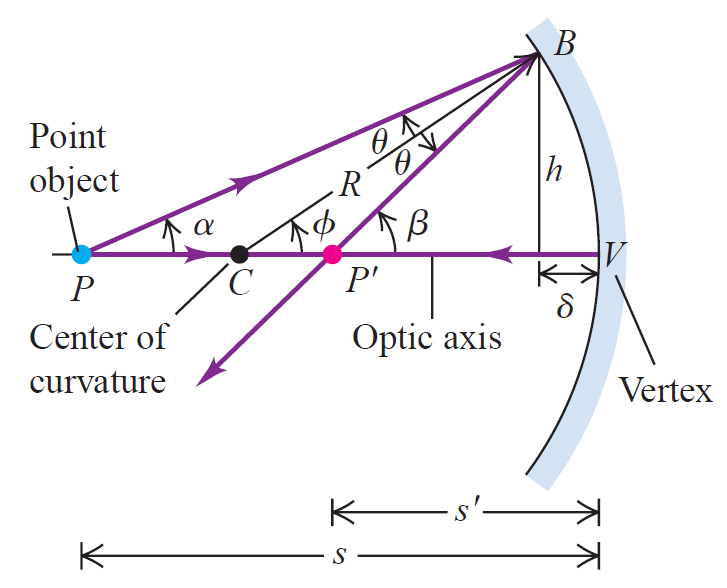
\includegraphics[scale=0.3]{Geometrisk-Optik/billeddannelse_krum.PNG}
	\caption{På figuren ses et punkobjekt placeret i punktet $P$ samt billedet af dette punktobjekt placeret i punktet $P'$ dannet ved et hulspejl.}
	\label{billeddannelse_krum}
\end{figure}
%
På samme måde som i \eqref{obj_img_fladt} vil man gerne finde en sammenhæng mellem objekt- og billedafstanden $s$ og $s'$. Dette kan gøres ved at lave nogle geometriske overvejelser ud fra figur \ref{billeddannelse_krum}. Kigger man først på trekanten $PBC$, ses det fra figuren at\footnote{Her angives vinklerne i radianer. Man finder en vinkel i radianer ud fra vinklen i grader ud fra formlen: $v_{\text{rad}} =  \pi \cdot \left( v_{\text{grad}} /180 \degree \right)$}
$$\pi = \alpha + \theta + x \, ,$$
hvor $x$ er den stumpe vinkel ved krumningscentrummet $C$. Dette siger blot, at alle tre vinkler i trekanten $PBC$ summer op til $\pi$ radianer (altså 180 grader). Man kan da bemærke, at vinklen $x$ i trekant $PBC$ og vinklen $\phi$ i trekant $CBP'$ til sammen udspænder $\pi$ radianer. Det betyder at
$$\pi = x + \phi \qquad \Rightarrow \qquad x = \pi - \phi$$
Sætter man dette ind i den ovenstående ligning, finder man da at
$$\phi = \alpha + \theta$$
På samme måde kan man kigge på trekanten $CBP'$, hvor man ved lignende overvejelser finder at
$$\beta = \phi + \theta$$
Ud fra disse to resultater kan man løse to ligninger med fire ubekendte, hvilket giver en ligning der relaterer $\alpha$, $\beta$ og $\phi$
\begin{equation}
\alpha + \beta = 2 \phi
\label{a_b_phi}
\end{equation}
Husker man da på fortegnskonventionerne fra det forrige afsnit, ses det, at både $s$, $s'$ og $R$ er positive størrelser. Ideen er da, at kigge på tangens til vinklerne $\alpha$, $\beta$ og $\phi$, og at udtrykke disse vha. størrelserne fra figur \ref{billeddannelse_krum}. Husker man, at tangens til en vinkel i en retvinklet trekant, forskellig fra den rette vinkel, kan skrives som den modstående divideret med den hosliggende katete, finder man at
$$\tan \alpha = \frac{h}{s - \delta}, \quad \quad \tan \beta = \frac{h}{s' - \delta}, \quad \quad \tan \phi = \frac{h}{R - \delta}. $$
Disse tre ligninger er ikke lige til at løse, men hvis man antager, at vinklen $\alpha$ er lille, således at $\beta$ og $\phi$ også er små, kan man lave en approksimation af tangens. Rent fysisk svarer dette til tilfældet, hvor objektafstanden $s$ er meget større end højden af spejlet $h$. I forhold til approksimationen af tangens gælder det, at $\tan x \approx x$, hvis $x$ er lille og angivet i radianer. Det bemærkes videre, at $\delta$ også vil være lille i dette tilfælde, så den kan også ignoreres. Dette giver tre ligninger
$$\alpha = \frac{h}{s}, \quad \quad \beta = \frac{h}{s'}, \quad \quad \phi = \frac{h}{R}.$$
Sætter man dette ind i relationen \eqref{a_b_phi}, får man da at
\begin{equation}
\frac{1}{s} + \frac{1}{s'} = \frac{2}{R}
\label{obj_img_krum}
\end{equation}
Som det næste er det interessant at kigge på, hvad der sker, hvis man tager objektet og flytter det uendeligt (i praksis meget) langt væk fra spejlet. Fysisk vil dette betyde, at alle de indgående stråler bevæger sig parallelt med den optiske akse, som illustreret på figur \ref{focal_point_12} del A). I dette tilfælde vil $1/s = 0$, hvilket ifølge \eqref{obj_img_krum} må give at
$$\frac{1}{s'} = \frac{2}{R} \quad \quad \Rightarrow \quad \quad s' = \frac{R}{2}$$
Det viser, at alle indkommende stråler vil have den samme billedafstand $s'$, og altså vil alle de indgående stråler samle sig i et enkelt punkt $F$, som det også er vist på figur \ref{focal_point_12} del A). Dette punkt kaldes for spejlets brændpunkt, og afstanden fra dette  til spejlets vertex kaldes for spejlets brændvidde, der betegnes $f$. Her har man, at brændvidden er givet ved
\begin{equation}
f = \frac{R}{2}
\label{focal_point_eq}
\end{equation} 
Som det ses af denne ligning afhænger brændvidden $f$ kun af $R$, hvilket betyder at både brændvidden $f$ og placeringen af brændpunktet $F$ er uafhængige af objekt- og billedafstanden $s$ og $s'$. brændpunkter er altså karakteristisk egenskab for et givet spejl.\\
Et andet interessant tilfælde, er det hvor objektet placeres i brændpunktet $F$, hvilket betyder at objektafstanden bliver $s = f = R/2$. Sætter man dette ind i \eqref{obj_img_krum} finder man således at
$$\frac{R}{2} + \frac{1}{s'} = \frac{R}{2} \quad \quad \Rightarrow \quad \quad \frac{1}{s'} = 0 \quad \quad \Rightarrow \quad \quad s' = \infty$$
Det viser, at billedet ligger uendeligt langt væk, således at alle de udgående lysstråler vil være parallelle med den optiske akse, som det er illustreret i figur \ref{focal_point_12} del B). Nu hvor brændvidden er blevet indført, er det mere konventionelt at skrive formel \eqref{obj_img_krum} på følgende form
\begin{equation}
\frac{1}{s} + \frac{1}{s'} = \frac{1}{f}
\label{ny_focal_s_s'}
\end{equation}

\begin{figure}[h!]
	\centering
	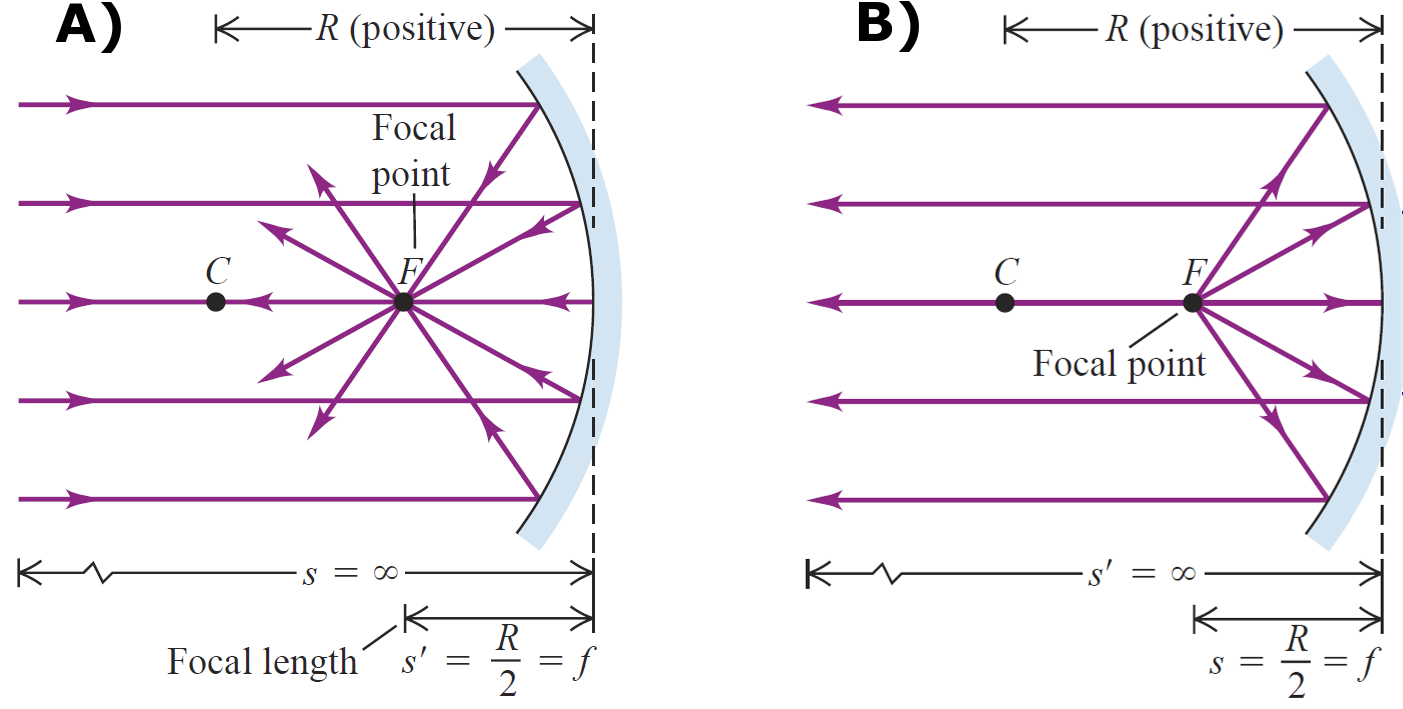
\includegraphics[scale=0.24]{Geometrisk-Optik/focal_point_12.PNG}
	\caption{På figurens del A) ses tilfældet hvor et objekt er placeret uendeligt langt fra et hulspejl, og hvor brændpunktet er placeret i punktet $F$. På del B) ses tilfældet, hvor objektet er placeret i brændpunktet $F$.}
	\label{focal_point_12}
\end{figure}
Det næste spørgsmål man kan stille sig selv er nu, hvad der sker, hvis man i stedet for et punktobjekt valgte et objekt med en udstrækning. Et eksempel på dette er vist på figur \ref{spejl_krum_pil}. Det vigtigste at bemærke her er, at man får to ensvinklede trekanter $PQV$ og $P'Q'V$. Det betyder specielt, at forholdet mellem længden af siderne $PV$ og $P'V$, er det samme som for siderne $PQ$ og $P'Q'$. Fra dette får man således
\begin{equation}
m = \frac{y'}{y} = - \frac{s'}{s}
\end{equation}

\begin{figure}[h!]
	\centering
	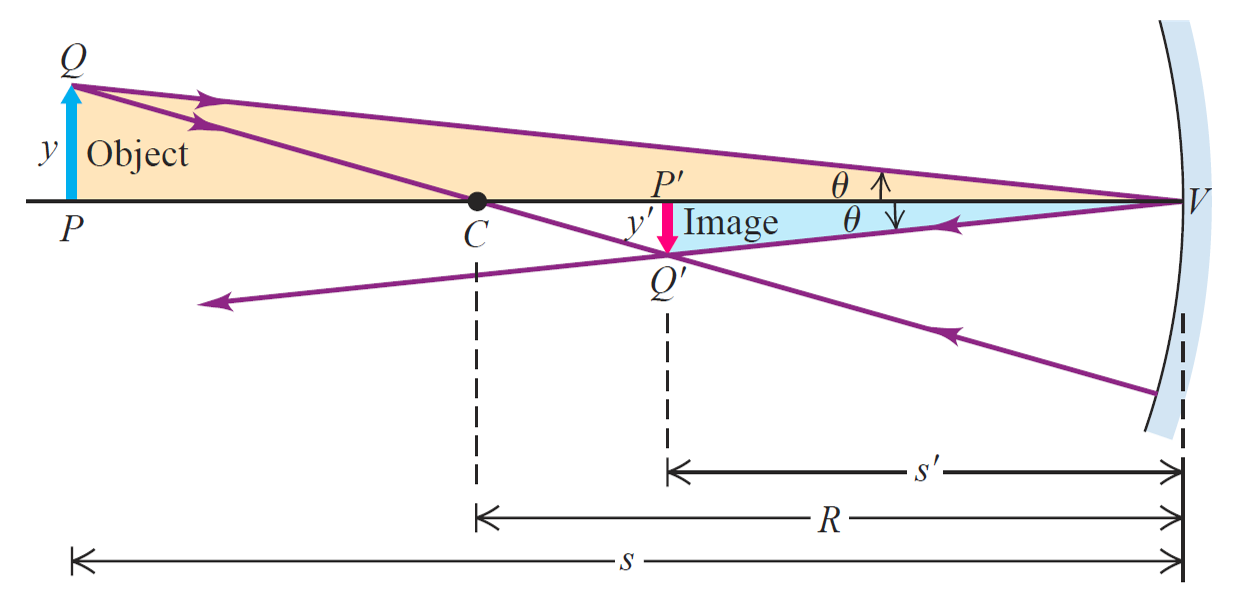
\includegraphics[scale=0.27]{Geometrisk-Optik/spejl_krum_pil.PNG}
	\caption{På figuren ses et eksempel på refleksion af et objekt med en udstrækning ved et hulspejl.}
	\label{spejl_krum_pil}
\end{figure} 
Nu hvor de fleste egenskaber ved refleksion fra et hulspejl er dækket, kan man kigge på hvad der sker, hvis man i stedet tager et såkaldt konvekst spejl, som er et spejl, der krummer væk fra observatoren i stedet for imod. To eksempler, hvor det ene er med et punktobjekt, og det andet er et objekt med en udstrækning, er vist på figur \ref{konveks_spejl}. På del A) af figuren kan man se, at krumningsradiusen $R$ her vil være negativ. Man kan da bruge den samme metode som for hulspejlet til at vise, at man her har relationen
\begin{equation}
\frac{1}{s} + \frac{1}{s'} = \frac{2}{R}
\end{equation}
På samme måde kan man også vise at
\begin{equation}
m = \frac{y'}{y} = - \frac{s'}{s}
\label{ref_for_jacob}
\end{equation}

\begin{figure}[h!]
	\centering
	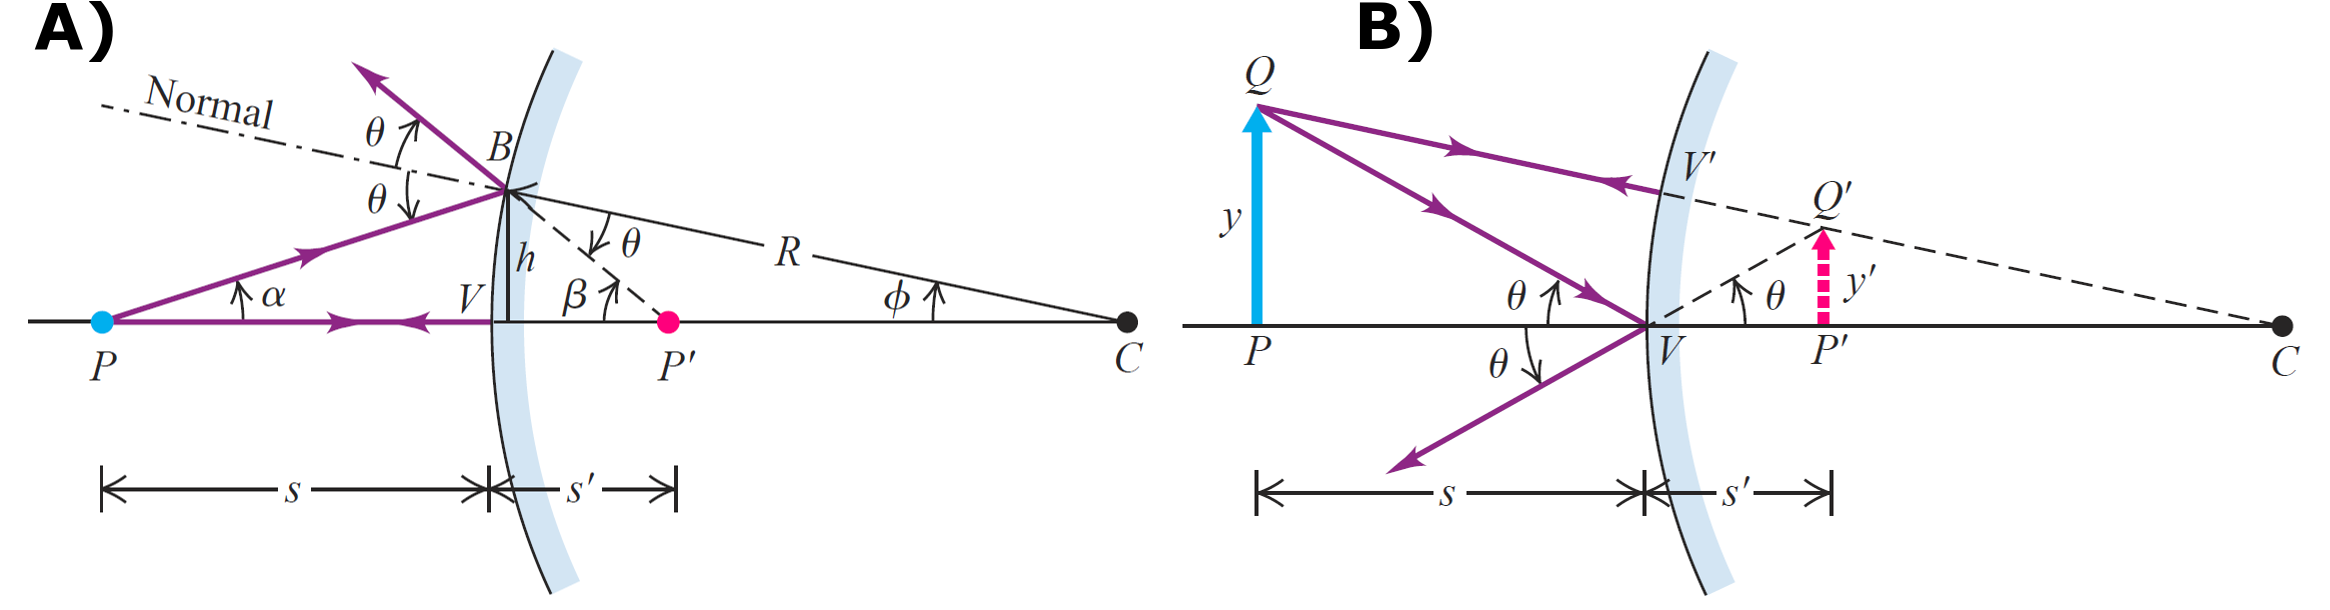
\includegraphics[scale=0.195]{Geometrisk-Optik/konveks_spejl.PNG}
	\caption{På figurens del A) ses et punktobjekt placeret i $P$, der ved refleksion ved et konvekst spejl danner billedet i $P'$. På del B) ses et objekt med en udstrækning, der også danner et billede ved refleksion.}
	\label{konveks_spejl}
\end{figure}
Ligesom for hulspejlet kan man også tale om brændpunkter og brændvidder for konvekse spejle. Kigger man på situationen i figur \ref{konveks_spejl2} del A), hvor de indkommende lysstråler er parallelle med den optiske akse, vil de ikke samle sig i et brændpunktet på samme måde, som det var tilfældet for hulspejlet. Til gengæld vil de udgående lysstråler se ud som om, at de kommer fra brændpunktet $F$ i en afstand $f$ bag spejlet. Her kalder man $f$ for brændvidden og $F$ for et virtuelt brændpunkt. Man finder også på samme vis som før at 
$$f = \frac{R}{2}$$
Den overordnede pointe er altså, at formlerne \eqref{spejl_krum_pil}, \eqref{obj_img_krum}, \eqref{focal_point_eq} og \eqref{ny_focal_s_s'} holder både for hulspejle og konvekse spejle, så længe man husker at bruge fortegnsreglerne for $s$, $s'$ og $R$ rigtigt.  
\begin{figure}[h!]
	\centering
	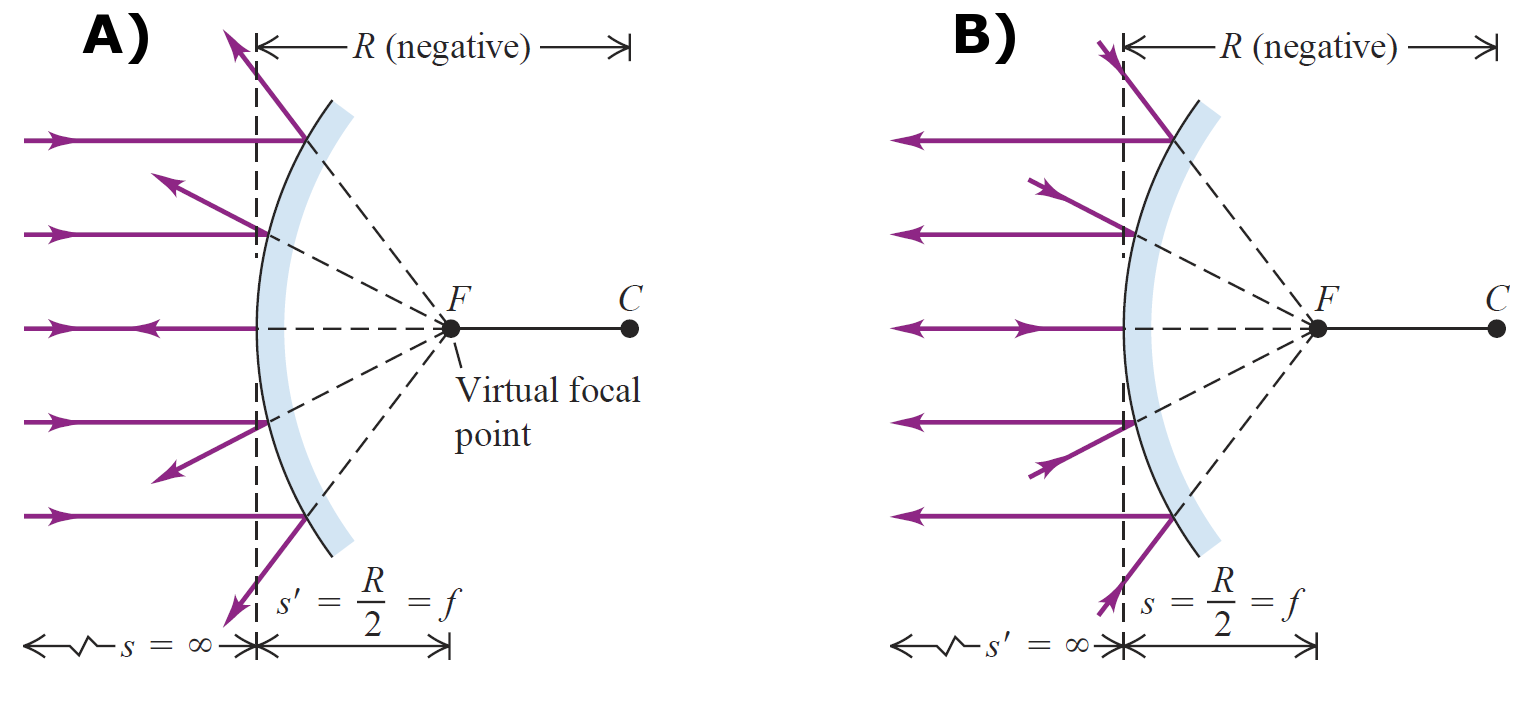
\includegraphics[scale=0.23]{Geometrisk-Optik/konveks_spejl2.PNG}
	\caption{På figurens del A) ses situationen, hvor objektet er placeret uendeligt langt væk fra spejlet. På del B) ses situationen, hvor objektet er placeret i det virtuelle brændpunkt $F$.}
	\label{konveks_spejl2}
\end{figure}
Før man går videre og kigger på, hvordan man kan bruge geometrisk optik til at beskrive linser, er det værd først at kigge på billeddannelse ved brydning for en krum overflade i stedet for ved refleksion, som det er gjort indtil nu. Et eksempel på dette, med et punktobjekt, er givet i figur \ref{konveks_brydning}. Det første man gerne vil, er at finde relationen mellem objekt- og billedafstanden. Dette kan igen gøres ved at lave nogle geometriske overvejelser. Kigger man først på trekanterne $PBC$ og $P'BC$, finder man at
$$\theta_a = \alpha + \phi \quad \quad \quad \quad \phi = \beta + \theta_b$$
Det næste man kan gøre, er da at bruge formel \eqref{bryd_lov} sammen med tangens til vinklerne $\alpha$, $\beta$ og $\phi$. Dette giver følgende udtryk
$$n_a \sin \theta_a = n_b \sin \theta_b \quad \quad \tan \alpha = \frac{h}{s + \delta} \quad \quad \tan \beta = \frac{h}{s' + \delta} \quad \quad \tan \phi = \frac{h}{R - \delta}$$
Det næste trin herfra er at antage, at $\alpha$ er lille, da det vil betyde, at alle de andre vinkler også er små. Derfor kan man lave en approksimation af både sinus og tangens til de forskellige vinkler, og bruge at $\delta$ bliver lille i forhold til $s$ og $s'$, så den også kan ignoreres. Det giver
$$n_a \theta_a = n_b \theta_b \, , \quad \quad \alpha = \frac{h}{s} \, , \quad \quad \beta = \frac{h}{s'} \, , \quad \quad \phi = \frac{h}{R} \, . $$
Bruger man udtrykket for $\theta_a$ fra før finder man da at
$$ \theta_b = \frac{n_a}{n_b} \left( \alpha + \phi \right) \, ,$$
og man kan da sætte det ind i udtrykket for $\phi$ fra før og få
$$\phi = \beta +  \frac{n_a}{n_b} \left( \alpha + \phi \right) \quad \quad \Rightarrow \quad \quad n_a\alpha + n_b \beta = \phi \left( n_b - n_a \right)$$
Endeligt kan man sætte de nye udtryk for $\alpha$, $\beta$ og $\phi$ ind i denne formel, hvilket giver det endelige resultat
\begin{equation}
\frac{n_a}{s} + \frac{n_b}{s'} = \frac{n_b - n_a}{R} 
\label{ref_til_jacob2}
\end{equation}
\begin{figure}[h!]
	\centering
	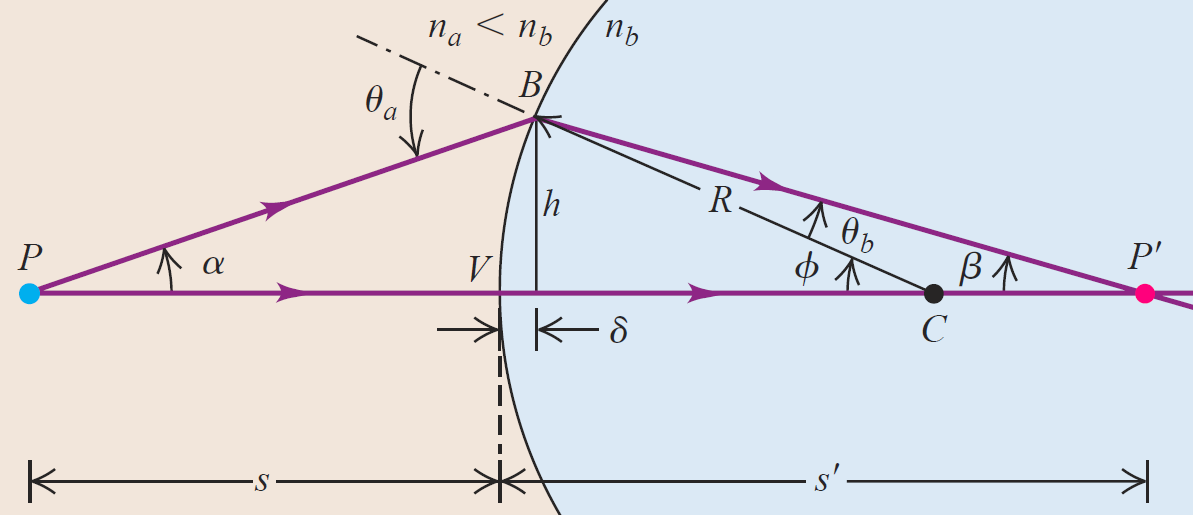
\includegraphics[scale=0.27]{Geometrisk-Optik/konveks_brydning.PNG}
	\caption{Figuren viser et eksempel på billeddannelse af et punktobjekt ved et konvekst spejl.}
	\label{konveks_brydning}
\end{figure}

Det sidste man gerne vil finde er forstørrelsen, når man har et objekt med en udstrækning. Dette gøres ved at betragte opsætningen på figur \ref{konveks_brydning2}. Det første man kan bemærke er, at man for trekanterne $PQV$ og $P'Q'V$ får
$$\tan \theta_a = \frac{y}{s} \, , \quad \quad \quad \quad \tan \theta_b = - \frac{y'}{s'} \, .$$
Fra \eqref{bryd_lov} får man også at
$$n_a \sin \theta_a = n_b \sin \theta_b$$
Så bruges det, at man for små vinkler har, at $\sin \theta \approx \tan \theta$, så man samlet set får at
$$\frac{n_a y}{s} = - \frac{n_b y'}{s'} \, ,$$
eller efter en lille omskrivning
\begin{equation}
m = \frac{y'}{y} = - \frac{n_a s'}{n_b s}
\end{equation}

\begin{figure}[h!]
	\centering
	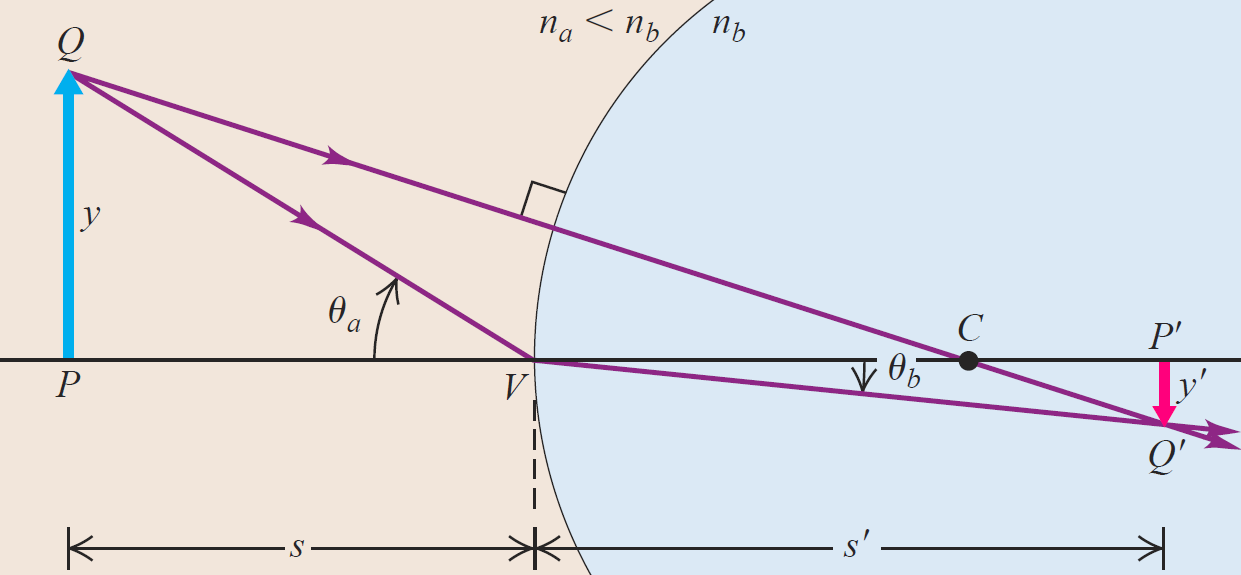
\includegraphics[scale=0.26]{Geometrisk-Optik/konveks_brydning2.PNG}
	\caption{Figuren viser et eksempel på billeddannelse af et objekt med en udstrækning ved et konvekst spejl.}
	\label{konveks_brydning2}
\end{figure} 

\section{Linser}
Vi vil i dette kapitel kigge nærmere på et af de mest brugte optiske værktøjer (efter det flade spejl), den tynde linse. Tynde linser bliver brugt i et utal af forskellige forsøgsopstillinger, så som optik, laser fysik og astronomi, og er derfor yderst interessante at undersøge

\subsection{Tynde linser}

En linse er et optisk system bestående af to brydende overflader, hvor den tynde linse består af to sfæriske overflader tæt nok på hinanden til, at afstanden imellem dem er negligerbar. I dette afsnit vil der blive gjort brug af resultaterne fra forrige afsnit omkring brydning ved sfæriske overflader. Der bruges herudover samme fortegnsregler som defineret tidligere. \\

\begin{wrapfigure}{r}{6cm}
	\centering
	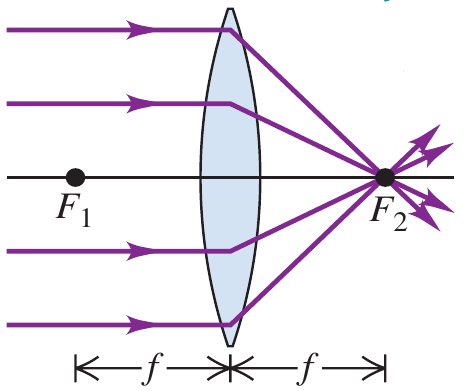
\includegraphics[width=4.5cm]{Geometrisk-Optik/conv_lens.PNG}
	\caption{Konvergerende tynd linse med brændpunkter $F_1$, $F_2$ og brændvidde $f$. } \label{fig:konv}
\end{wrapfigure}

\noindent En linse af formen vist i figur \ref{fig:konv} har den egenskab, at når stråler parallel til den optiske akse passerer igennem linsen, dannes der et billede ved punktet $F_2$. Omvendt, så vil stråler udsendt fra $F_1$ være parallelle til aksen efter at have passeret igennem linsen. Denne type af linse kaldes for en konvergerende linse. Punkterne $F_1$ og $F_2$ kaldes for hhv. det første og andet brændpunkt, mens afstanden $f$ (målt fra centrum af linsen) kaldes for brændvidden. For en konvergerende linse er brændvidden $f$ positiv. Bemærk her ligheden med det krumme spejl fra forrige kapitel. \\ 

\noindent Ligesom ved det krumme spejl, kan et konvergerende spejl danne et billede af et udstrakt objekt. Lad $s$ og $s'$ betegne hhv. objekt- og billedeafstanden og $y$ og $y'$ betegne hhv. objekt- og billedehøjden. På figur \ref{bla} ses strålen $QA$ brydes igennem $F_2$, mens strålen $QO$ passerer igennem uden at ændre retning, da vi har antaget at vi arbejder med en tynd linse, hvor overfladerne i centrum er parallelle. Vinklerne $\alpha$ er her ens, og derved må forholdet mellem siderne i trekanterne $PQO$ og $P'Q'O$ også være det,
\begin{equation}
\frac{y}{s} = -\frac{y'}{s'} \quad \text{eller} \quad \frac{y'}{y} = -\frac{s'}{s},
\label{eq:1}
\end{equation}

\noindent hvor det negative fortegn skyldes, at billedet er under den optiske akse. Vinklerne $\beta$ er også ens, hvilket medfører at forholdet mellem siderne i trekanterne $OAF_2$ og $P'Q'F_2$ også er ens, hvorved

\begin{equation}
\frac{y}{f}=-\frac{y'}{s'-f} \quad \text{eller} \quad \frac{y'}{y} = -\frac{s'-f}{f}
\label{eq:2}
\end{equation}

\noindent Ud fra ligning \eqref{eq:1} og ligning \eqref{eq:2} får vi relationen

\begin{equation}
\frac{1}{s}+\frac{1}{s'} = \frac{1}{f} \, ,
\label{eq:3}
\end{equation}

\noindent hvilket er den samme relation mellem objekt og billede, vi fandt for det konvekse spejl i ligning \eqref{ny_focal_s_s'}. Vi får herudover også et udtryk for den tværgående forstørrelse, ækvivalent til ligning \eqref{ref_for_jacob},

\begin{equation}
m = \frac{y'}{y} = -\frac{s'}{s}
\label{eq:4}
\end{equation}

\begin{figure}[h!]
	\centering
	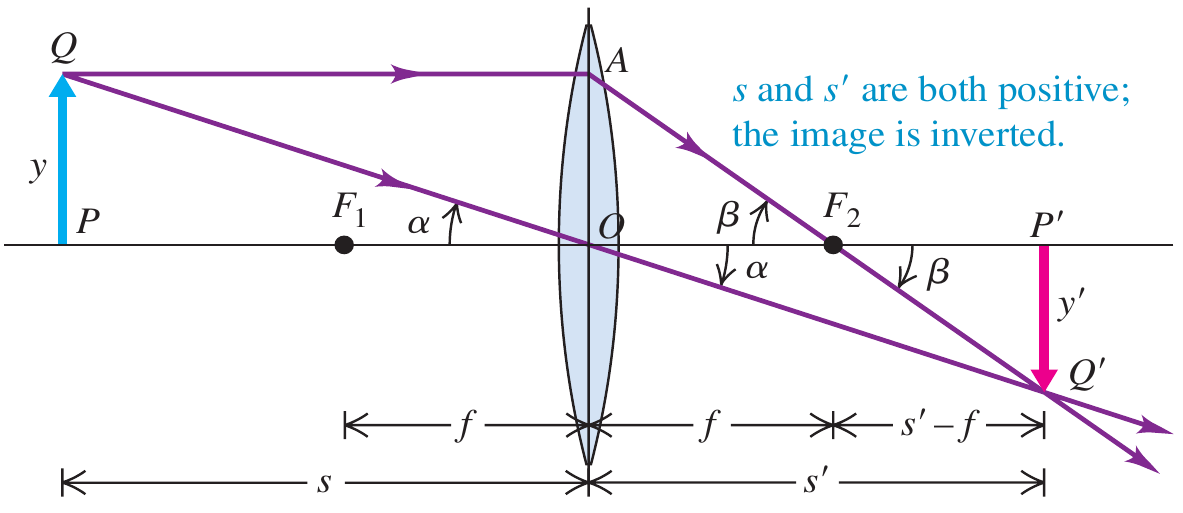
\includegraphics[scale=0.3]{Geometrisk-Optik/lens_objekt.PNG}
	\caption{Model til at finde objekt position for en tynd linse.}
	\label{bla}
\end{figure}

\noindent De to ovenstående ligninger er grundligningerne for tynde linser, og er som sagt af samme form som de tidligere fundne ligninger for sfæriske spejle. Det negative fortegn i ligning \eqref{eq:4} betyder, at når $s$ og $s'$ er positive, så vil billedet være inverteret , og $y$ og $y'$ vil have modsatte fortegn. Hvis vi antager at $f>0$ (en konvergerende linse), så giver ligning \eqref{eq:3} os, at når objektet er uden for det første brændpunkt $F_1$ ($s>f$) vil billedeafstanden $s'$ være positiv og billedet inverteret. Når billedeafstanden er positivt, er billedet per definition på den modsatte side af linsen end objektet, og kaldes for reelt. Omvendt så vil et objekt placeret inden for det første brændpunkt ($s<f$) danne et billede med negativ billedeafstand $s'$. Dette billede er ikke-inverteret, og placeret på samme side af linsen som objektet. Når billedeafstanden er negativ, og billedet befinder sig på samme side af linsen som objektet, kaldes billedet for virtuelt.

\newpage

\begin{wrapfigure}{r}{6cm}
	\centering
	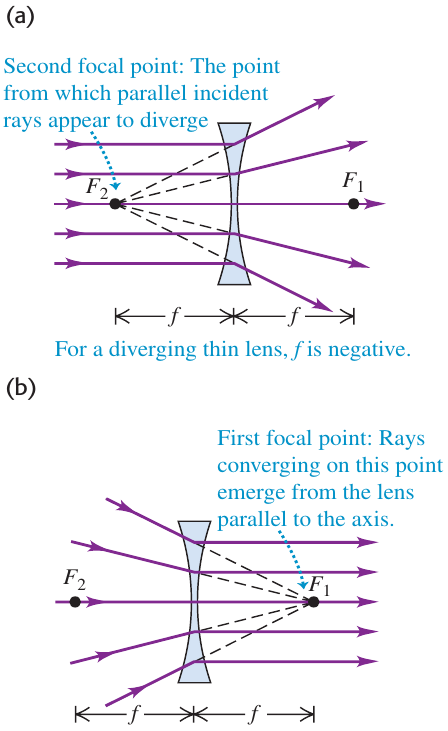
\includegraphics[width=5cm]{Geometrisk-Optik/div_lens.PNG}
	\caption{Divergerende linse med negativ $f$, og brændpunkter $F_1$ og $F_2$.}
	\label{div}
\end{wrapfigure}

\noindent I figur \ref{div} vises en divergerende linse, en anden form for tynd linse. Lysstråler parallelle til den optiske akse divergere efter brydning. Brændvidden $f$ for divergerende linser er en negativ størrelse, mens brændpunkterne $F_1$ og $F_2$ er modsat placeret i forhold til den konvergerende linse. Parallelle stråler der brydes lader til at være udsendt fra punktet $F_2$, mens stråler der konvergerer mod punktet $F_1$ er parallelle til den optiske akse efter brydning, som set i hhv. figur \ref{div}a og figur \ref{div}b. Ud fra dette kan vi se at divergerende linser har det samme forhold til konvergerende linser, som konvekse spejle havde til konkave spejle i forrige kapitel. Man ville kunne foretage den samme geometriske analyse som tidligere i dette kapitel, for at vise at ligning \eqref{eq:3} og \eqref{eq:4} også er gældende for divergerende linser.\\

\subsection{Linsemagerens ligning}
\noindent Ud fra analysen af tynde linser påstår vi følgende, \\

\noindent \textsl{Enhver linse der er tykkere på midten end ved kanterne er en konvergerende linse, og enhver linser der er tykkere ved kanterne end på midten er en divergerende linse.} \\


\noindent Denne påstand kan vises ved at lave en dybdegående udledning af ligning \eqref{eq:3}, hvorved vi også vil udlede \textsl{Linsemagerens ligning}. Denne ligning beskriver forholdet mellem brændvidde $f$, linsens brydnings index $n$, og overfladernes radiusser $R_1$ og $R_2$. Vi starter generelt ud med en bi-konvergerende linse (bedre kendt som en bi-konveks linse) med tykkelse $t$ og med brydningsindeks $n_2$ omkredset af et materiale med brydningsindeks $n_1$, illustreret i figur \ref{bikonv}. De to sfæriske overflader har hhv. radiuserne $R_1$ og $R_2$. Vi betragter punktobjektet $P$, med objektafstand $s_1$ fra den første overflade. Lysstråler udsendt fra $P$ brydes af den første overflade og danner et virtuelt billede $Q'$ med billedeafstand $s'_1$. Ud fra de definerede fortegnskonventioner er $s_1>0$, $s_1'<0$ og $R_1>0$. Ud fra ligning \eqref{ref_til_jacob2} får man følgende relation,
\begin{equation}
\frac{n_1}{s_1}+\frac{n_2}{s'_1} = \frac{n_2-n_1}{R_1}
\label{eq:5}
\end{equation}

\noindent Det virtuelle billede $Q'$ danner nu et objekt med objektafstand $s_2 = \abs{s'_1}+t = t-s'_1$ for den anden sfæriske overflade. Stråler fra $Q'$ brydes og danner et reelt billede $Q$ med billedafstand $s'_2$. Her har vi at $s_2>0$, $s'_2>0$ og $R_2 < 0$. Vi kan da opstille relationen

\begin{equation}
\frac{n_2}{s_2}+\frac{n_1}{s'_2} = \frac{n_1}{s'_2} + \frac{n_2}{t-s'_1} = \frac{n_1-n_2}{R_2}
\label{eq:6}
\end{equation}

\begin{figure}[h!]
	\centering
	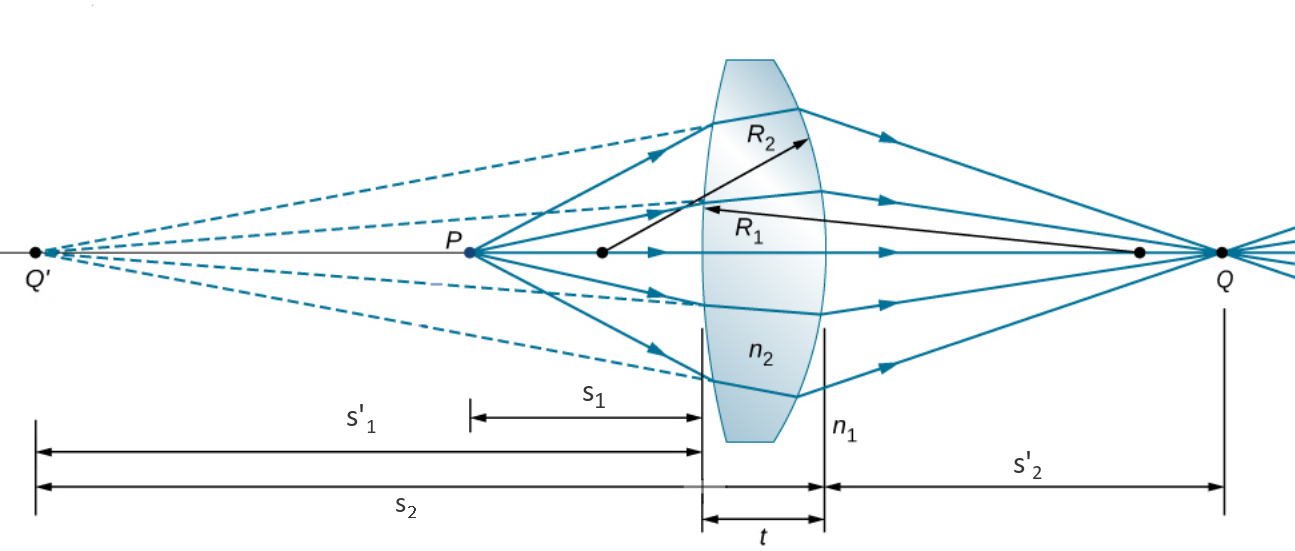
\includegraphics[scale=0.3]{Geometrisk-Optik/lensmaker.PNG}
	\caption{Brydning af lys igennem en bi-konveks linse med tykkelse $t$.}
	\label{bikonv}
\end{figure}


\noindent Ved at addere ligning \eqref{eq:5} og ligning \eqref{eq:6} får vi

\begin{equation}
\frac{n_1}{s_1}+\frac{n_2}{s'_1} + \frac{n_1}{s'_2} + \frac{n_2}{t-s'_1} = (n_2 - n_1) \left( \frac{1}{R_1} - \frac{1}{R_2} \right)
\end{equation}

\noindent For tynde linser er det gældende at $t\ll s'_1$, hvorved man får

\begin{equation}
\frac{1}{s_1}+\frac{1}{s'_2} = \left(\frac{n_2}{n_1}-1\right)\left( \frac{1}{R_1}-\frac{1}{R_2} \right)
\end{equation}

\noindent Her kan $s_1$ betragtes som objektafstanden $s$, $s'_2$ kan betragtes som billedeafstanden $s'$, og da vi oftest betragter linser i luft kan vi sætte $n_1=1$ og $n_2=n$, hvorved vi får følgende vha. ligning \eqref{eq:3}

\begin{equation}
\frac{1}{f} = \frac{1}{s} + \frac{1}{s'} = (n-1)\left( \frac{1}{R_1} - \frac{1}{R_2}\right)
\end{equation}

\noindent Den ovenstående ligning kaldes for Linsemagerens ligning, som er gældende for alle tynde linser. Ved brug af de definerede fortegnsregler, kan den tidligere påstand omkring konvergerende og divergerende linser vises, da linser der er bredere ved midten vil resultere i en positiv brændvidde, mens linser der er bredere ved enderne vil resultere i en negativ brændvidde. 

